\documentclass[boxes]{gsypset}

% Info for header
\mailbox{}
\initials{}
\collaborators{}
\class{Math 60}
\assignment{HW 7}
\duedate{May 25, 2016}

\usepackage{caption}

\begin{document}
	\begin{problem}[4.2.28]
		Show that the largest rectangular box having a fixed surface area must be a cube.
	\end{problem}
	\begin{solution}
		
	\end{solution}
	
	\begin{problem}[4.2.30]
		Find the points on the surface $xy + z^2 = 4$ that are closest to the origin.
		Be sure to give a convincing argument that your answer is correct.
	\end{problem}
	\begin{solution}
		
	\end{solution}
	
	\begin{problem}[4.2.34]
		A metal plate has the shape of the region $x^2 + y^2 \geq 1$.
		The plate is heated so that the temperature at any point $(x,y)$ on it is indicated by
		\[
			T(x,y) = 2x^2 + y^2 - y + 3
		\]
		Find the hottest and coldest points on the plate and the temperature at each of these points.
		(Hint: Parameterize the boundary of the plate in order to find any critical points there.)
	\end{problem}
	\begin{solution}
		
	\end{solution}
	
	\begin{problem}[4.2.46]
		\[
			f(x,y) = e^{x^2 + 5y^2}
		\]
		\begin{subproblems}
			\subproblem Find all critical points of $f$ and identify their nature as local extrema.
				\begin{solution}
					
				\end{solution}
				
			\subproblem Determine, with explanation, any global extrema of $f$.
				\begin{solution}
					
				\end{solution}
		\end{subproblems}
	\end{problem}
	
	\begin{problem}[4.3.6]
		Use Lagrange multipliers to identify the critical points of
		\[
			f(x,y,z) = x^2 + y^2 + z^2
		\]
		subject to the constraint
		\[
			x+y-z = 1
		\]
	\end{problem}
	\begin{solution}
		
	\end{solution}
	
	\begin{problem}[4.3.24]
		You are sending a birthday present to your calculus instructor. 
		Fly-By-Night Delivery Service insists that any package it ships be such that 
		the sum of the length plus the girth be at most \SI{108}{in}. 
		(The girth is the perimeter of the cross section perpendicular to the length axis
		--- see Figure 4.31.) 
		What are the dimensions of the largest present you can send?
		\begin{center}
			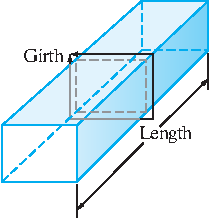
\includegraphics{img/4_3_24}
			\renewcommand{\thefigure}{4.31}
			\captionof{figure}{Diagram for Exersize 24.}
		\end{center}
	\end{problem}
	\begin{solution}
		
	\end{solution}
	
	\begin{problem}[4.3.26]
		An industrious farmer is designing a silo to hold her 
		\SI[parse-numbers=false]{900\pi}{ft^3} supply of grain. 
		The silo is to be cylindrical in shape with a hemispherical roof. 
		(See Figure 4.32.) 
		Suppose that it costs five times as much (per square foot of sheet metal used) 
		to fashion the roof of the silo as it does to make the circular floor and 
		twice as much to make the cylindrical walls as the floor. 
		If you were to act as consultant for this project, 
		what dimensions would you recommend so that the total cost would be a minimum? 
		On what do you base your recommendation? 
		(Assume that the entire silo can be filled with grain.)
		\begin{center}
			
\includegraphics{img/4_3_26}
			\renewcommand{\thefigure}{4.32}
			\captionof{figure}{The grain silo for Exersize 26.}
		\end{center}
	\end{problem}
	\begin{solution}
		
	\end{solution}
\end{document}